\documentclass[11pt]{article}
\usepackage{graphicx}
\usepackage{caption}
\usepackage{subcaption}
\usepackage[a4paper, portrait, margin=1in]{geometry}

\usepackage{mathtools}
\DeclarePairedDelimiter{\ceil}{\lceil}{\rceil}

\begin{document}

\title{Advanced Systems Lab (Fall'16) -- Second
Milestone}

\author{Name: \emph{Aleksander Matusiak}\\Legi number: \emph{16-931-925}}

\date{
\vspace{4cm}
\textbf{Grading} \\
\begin{tabular}{|c|c|}
\hline  \textbf{Section} & \textbf{Points} \\ 
\hline  1 &  \\ 
\hline  2 &  \\ 
\hline  3 &  \\ 
\hline \hline Total & \\
\hline 
\end{tabular} 
}

\maketitle

\newpage

\section*{Notes on writing the report \small{(remove this page for submission)}}

Before starting to work on this milestone please remember:
\begin{itemize}
\item The prerequisite to a successful completion to this milestone is to have a stable system and also the necessary logging functionalities in place. 
\item Depending on the workload and goal of the experiment, you might need to change the sampling rate from the default level. Make sure to indicate when doing so.
\item The choice of experiment length and repetitions is up to you to decide, please make sure that you do not include warm-up and cool-down phases in the measurements. There are many experiments to run in this milestone, try to make a tradeoff.  
\item We recommend that you have scripts in place to deploy and run experiments.
\item All experiments have to be executed on the Microsoft Azure cloud.
\item When plotting graphs include errors or measures of accuracy whenever possible. 
\item Keep the report compact and concise! The total length should not exceed 20 pages. Log listings are not counted in this length, but all text, figures and tables are. If you have many logs, compress them by experiment and reference the archive instead of the independent files.
\end{itemize}

In this milestone we expect to see the different experiments you ran to exercise the system, and with each experiment we expect a clear description of the system configuration used, the hypothesis on behavior and the explanation of the behavior observed (in terms of the different design decisions taken beforehand) -- \emph{missing either of these for an experiment might make you lose all points for that given experiment!} 

Keep in mind that for a good explanation of the results of an experiment you might have to use one or more methods of data analysis presented in the lecture and in the book. You might have to combine measurements taken in the middleware with the ones at the clients to be able to provide a full picture.

Please feel free to structure the three sections of this report as it makes most sense for your experiments and explanations, but please respect the goal of each section. Also, similarly to the first milestone, include tables and descriptions about your experimental setup before each set of experiments.


\pagebreak

\section{Maximum Throughput}

%Find the highest throughput of your system for 5 servers with no replication and a read-only workload configuration. What is the minimum number of threads and clients (rounded to multiple of 10) that together achieve this throughput? Explain why the system reaches its maximum throughput at these points and show how the performance changes around these configurations. Provide a detailed breakdown of the time spent in the middleware for each operation type.

\subsection{Hyphotesis}

The throughput, as we increase the number of clients, should be increasing, at least to the point where my middleware encounters problem. However, as we could already see on the plot for baseline experiment in the milestone 1, the mean response time shall increase almost in a linear way. This means that the maximal effective throughput will be probably achieved for not that big number of clients - for higher number of clients throughput will probably still increase slightly, but the response time would increase much faster.

The throughput, as we increase the number of threads in the thread pool, should also be increasing. However, creating more threads is associated with more overhead from operating system and might not improve the throughput as much as we would expect. 

I predict that the bottleneck for the middleware would be the receiving of incoming client requests and putting them into an appropriate queue, since it is performed by only one thread, while every other operation can be executed by multiple threads in parallel. This means that at some points increasing the number of threads in the thread pool would not affect the throughput significantly - it will be limited by the bottleneck, which isn't affected by the increase of threads.
%TODO 

\subsection{General experimental setup}
Using memaslap in the read-only configuration means that before actual statistics are being displayed there is a phase where each memaslap clients sends only set requests in order to fill up the server with some keys, which it can later query. This face was initially taking a very longs time due to the default window size. Therefore, for all the experiments in this task I have decreased the window size for each memaslap client to 1k, which made initial phase with only set requests much shorter (lasting less than one minute). However, different servers still could finish initial phase much before others. Therefore, to be sure that during actual measurement all memaslap servers are sending only get requests, I have conducted the experiments for 5 minutes and for calculating statistics I have used only the third minute. This means 2 minutes for warm up phase and 2 minutes for cool down phase, which includes waiting with measurements for other servers to stop sending set requests. I have collected statistics every second. This means that for each configuration I have collected 60 numbers, from which I could calculate average, standard deviation and, when applicable, percentiles. Due to the limit of money I was able to use for this milestone (my subscription was renewed on 1st November), I couldn't afford repetition of the experiment. Even though I was left with some funds near the end of the milestone, conducting repetition experiments not immediately after the original one, would not give any positive contribution for my experiments, since the results would differ significantly due to uncertainty of the Azure cloud. However, I strongly believe that collecting 60 values for each configuration, as described above, provides statistical significance for my experiments.   

To avoid memcached misses I have increased the memory of each memcached server to 256 MB.

In order to enable distinction between between set and get requests in the middleware logs, I have added writing the type of request for every log entry. What is more, with higher number of clients, my middleware was sometimes not forwarding received requests and responses correctly. This was due to not checking for emptiness of the buffer after sending the first part of the message - sending should be continued till the buffer is empty. This bug was fixed in the source code and corrected code was used for running the experiments for this milestone. 

\subsection{Overall experiment}
This experiment was conducted using the following provided scheme:
\medskip

\small{
\smallskip
\begin{tabular}{|c|c|}
\hline Number of servers & 5 \\ 
\hline Number of client machines & 5 \\ 
\hline Virtual clients / machine & 20 - 100 \\ 
\hline Step for virtual clients / machine & 10 \\ 
\hline Threads in the thread pool & 10 - 60 \\
\hline Step for threads in the thread pool & 10 \\
\hline Workload & Key 16B, Value 128B, Writes 0\% \\
\hline Middleware & No replication \\ 
\hline Runtime x repetitions & 5 min x 1 \\ 

\hline Log files & overall1, overall2, overall3, overall4, overall5, overall \\
\hline 
\end{tabular} }
\medskip


\begin{figure}
\centering
\begin{subfigure}{.5\textwidth}
	\centering
	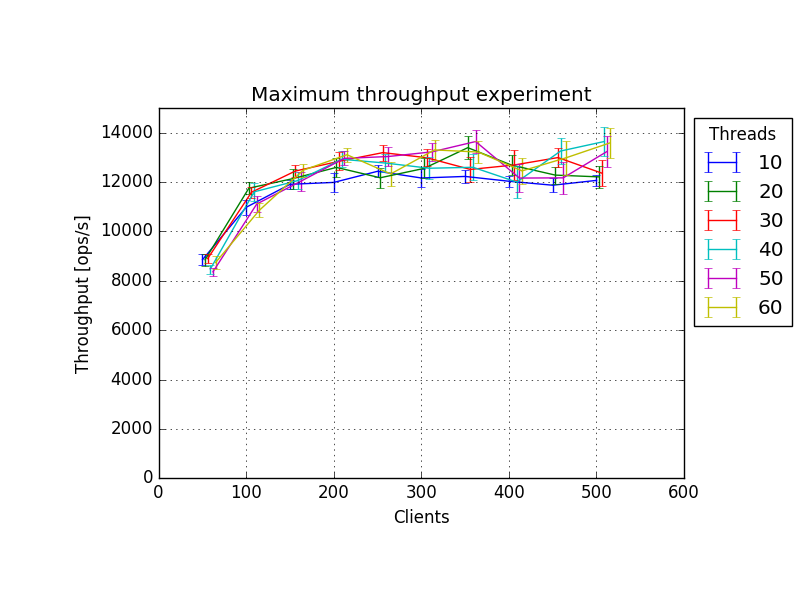
\includegraphics[width=\linewidth]{plots/max_throughput_all_overall}
	\caption{Throughput}
\end{subfigure}%
\begin{subfigure}{.5\textwidth}
	\centering
	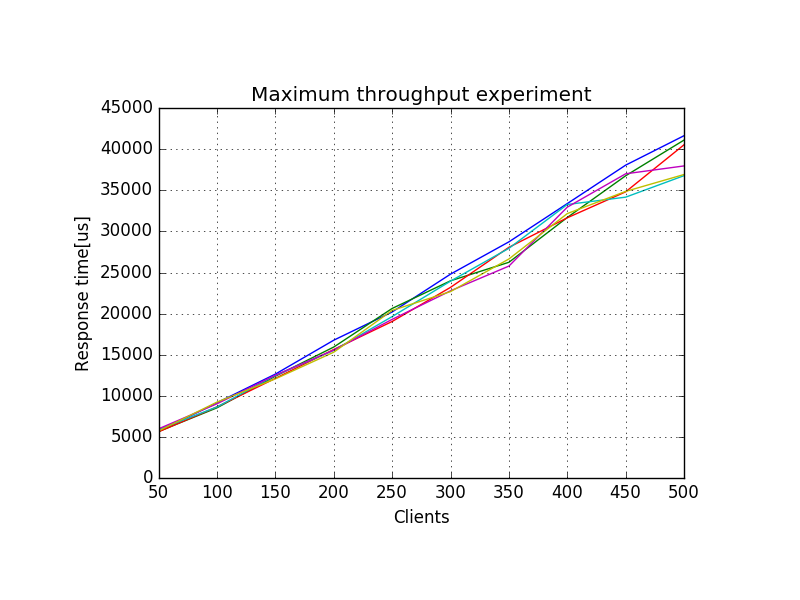
\includegraphics[width=\linewidth]{plots/max_throughput-response_time_all_overall}
	\caption{Response time}
\end{subfigure}
\caption{Plots for various number of threads in the overall experiment}
\label{fig:max-throughput-overall}
\end{figure}

Results of this experiments are visible in the figure \ref{fig:max-throughput-overall}.

As we can see from the plots, the throughput up to 500 clients is slightly growing. However, the response time is also growing in almost linear manner. This means that the maximal effective throughput should be achieved by clients in range around 150 - 250 clients. More precisely, the highest throughput for my experiment was achieved using 500 clients and 40 threads in the thread pool - it was equal to 13648 ops/s and it was corresponding to mean response time equals to around 36790 us. If we look at the range 150-250 clients, the highest throughput was achieved for 250 clients and 30 threads - it was equal to 13196 ops/s and it was corresponding to mean response time equals to around 19057 us. This means that by limiting our analysis to range till 250 clients, we get highest throughout worse by around 3,3\%, but the response time is around 48,2\% lower (better). This means that we can indeed concentrate on the number of clients till 250, since the increase of the number of clients above it will maybe slightly increase throughput, but the response time will grow significantly.

% TODO: interactive law

It must also be pointed out here that number of threads does not make such a big difference as one could expect. We can clearly see in the plot that the middleware having 10 threads in each of the thread pool is performing noticeably worse then the middleware having more threads. We can still see that below 300 clients the middleware with the thread pool of size 20 is performing less effective than with other configurations. However, for bigger number of clients and size of the thread pool, difference in performance is not really significant. Therefore, as the optimal number of threads I have chosen 30 threads, since lower number of threads results in noticeably lower performance and higher number of threads does not make a significant difference. The reason why this is the case is probably the bottleneck for the middleware is receiving incoming requests from the clients, not forwarding them to servers. This will be thoroughly analyzed in the subsection \ref{sec:time-breakdown}. What is more, the reason for not big effect of the number of threads might be the overhead from operating systems. Having more threads costs some system resources and since the virtual machine has only 8 cores, the threads might not be in reality performing task in parallel, but rather one after another.
% TODO: how many cores

\subsection{Detailed experiment}

This experiment was conducted using the following provided scheme:
\medskip

\small{
\smallskip
\begin{tabular}{|c|c|}
\hline Number of servers & 5 \\ 
\hline Number of client machines & 5 \\ 
\hline Virtual clients / machine &  20 - 60 \\ 
\hline Step for virtual clients / machine & 2 \\
\hline Workload & Key 16B, Value 128B, Writes 0\% \\
\hline Middleware & No replication \\ 
\hline Runtime x repetitions & 5 min x 1 \\ 
\hline Log files & TODO \\
\hline 
\end{tabular} }
\medskip

\begin{figure}
\centering
\begin{subfigure}{.5\textwidth}
	\centering
	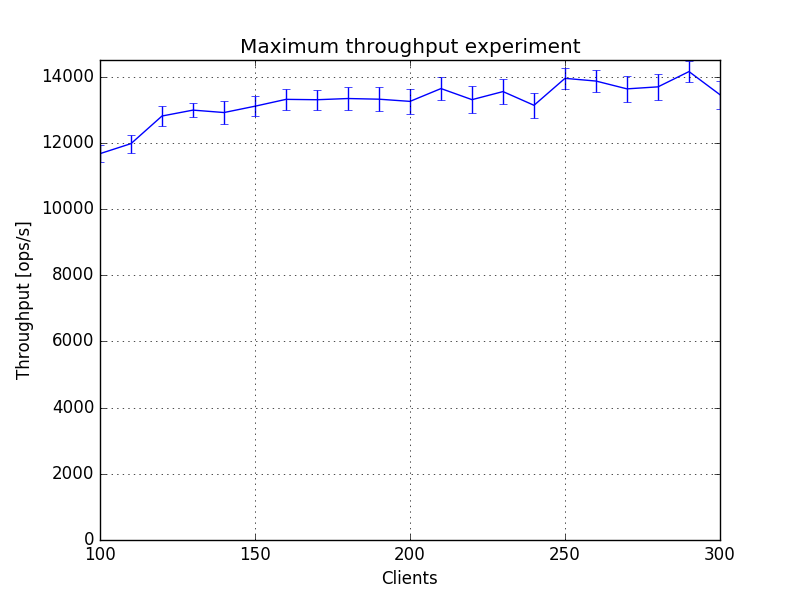
\includegraphics[width=\linewidth]{plots/max_throughput_all_detailed}
	\caption{Throughput}
\end{subfigure}%
\begin{subfigure}{.5\textwidth}
	\centering
	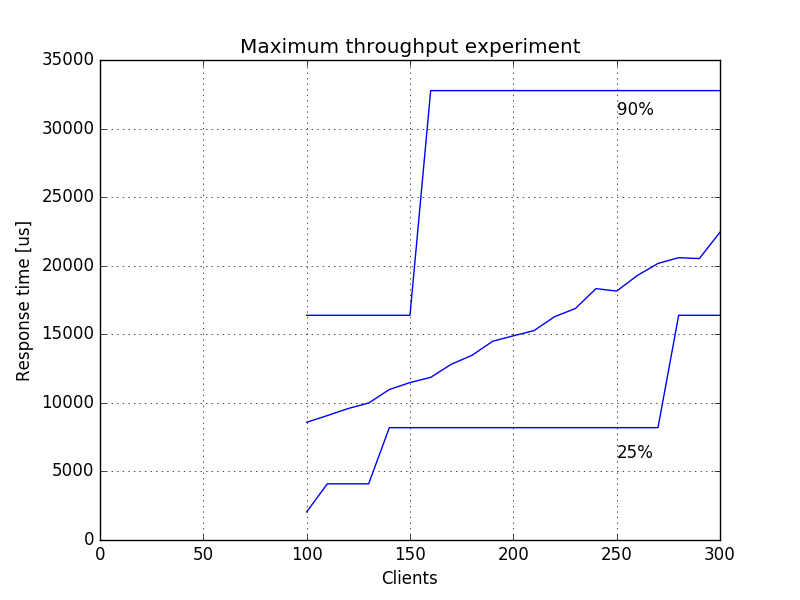
\includegraphics[width=\linewidth]{plots/max_throughput-response_time_all_detailed}
	\caption{Response time}
\end{subfigure}
\caption{Plots for various number of threads in the detailed experiment}
\label{fig:max-throughput-detailed}
\end{figure}

Results of this experiments are visible in the figure \ref{fig:max-throughput-detailed}.


To sum up, the maximal effective throughput is achieved for 210 clients and size of thread pool equals 30. Therefore, I will use this parameters in later experiments.  

\subsection{Verification of the hyphotesis}

As I have suspected, the number of clients for the maximal effective throughput was not that big and increasing number of clients further would only cause a slight increase in the throughput and a more significant increase in the mean response time. Further increasing of threads above 30 threads, as predicted, does not contribute to the higher throughput.

\subsection{Breakdown of the time spent in the middleware}
\label{sec:time-breakdown}

Since the purpose of this experiment was to analyze middleware under read-only workload, in this section I will provide breakdown of the time spent in the middleware for get operations.
\medskip

\begin{tabular}{|c|c|c|c|}
\hline \bf{Time spent ...} & \bf{Average (us)} & \bf{Standard deviation (us)} & \bf{Coefficient of variation} \\ 
\hline in the middleware & 6831 & 12834 & 1.88 \\
\hline in the queue & 2572 & 6962 & 2.71\\
\hline in the server & 4217 & 9994 & 2.37\\
\hline in the queue and the server & 6789 & - & -\\
\hline being actively processed & 42 & - & -\\
\hline
\end{tabular}
\medskip

\pagebreak

\section{Effect of Replication}

\iffalse
Explore how the behavior of your system changes for a 5\%-write workload with S=3,5 and 7 server backends and the following three replication factors:
\begin{itemize} 
\item Write to $1$ (no replication) 
\item Write to $\ceil{\frac{S}{2}}$ (half) 
\item Write to all 
\end{itemize}

Answer at least the following questions: Are \texttt{get} and \texttt{set} requests impacted the same way by different setups? If yes/no, why? Which operations become more expensive inside the middleware as the configuration changes? How does the scalability of your system compare to that of an ideal implementation? Provide the graphs and tables necessary to support your claims.
\fi

\subsection{Hyphotesis}

\subsection{Experimental setup}

\small{
\smallskip
\begin{tabular}{|c|c|}
\hline Number of servers & 3 - 7 \\ 
\hline Step for number of servers & 2 \\
\hline Number of client machines & 3 \\ 
\hline Virtual clients / machine &  70 \\ 
\hline Workload & Key 16B, Value 128B, Writes 5\% \\
\hline Middleware & Replication: none, half, all \\ 
\hline Runtime x repetitions & 3 min x 1 \\ 
\hline Log files & TODO \\
\hline 
\end{tabular} }
\medskip

\subsection{Overall performance}
\begin{figure}
\centering
	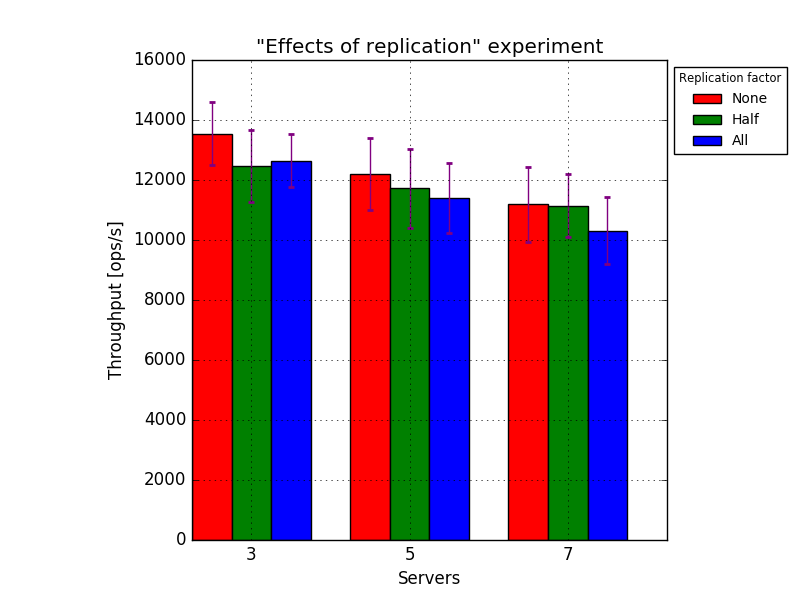
\includegraphics[width=0.7\linewidth]{plots/replication}

\caption{Aggregated throughput for the replication experiment}
\label{fig:replication-overall}
\end{figure}


\subsection{Get requests}
\begin{figure}
\centering
	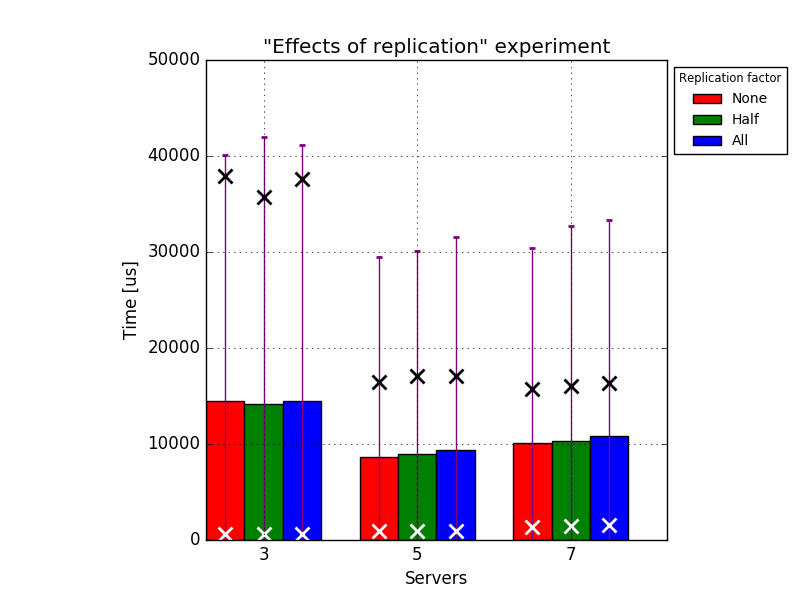
\includegraphics[width=0.7\linewidth]{plots/replication-get}

\caption{Total time spent in the middleware for get requests}
\label{fig:replication-get}
\end{figure}

\begin{figure}
\centering
\begin{subfigure}{.5\textwidth}
	\centering
	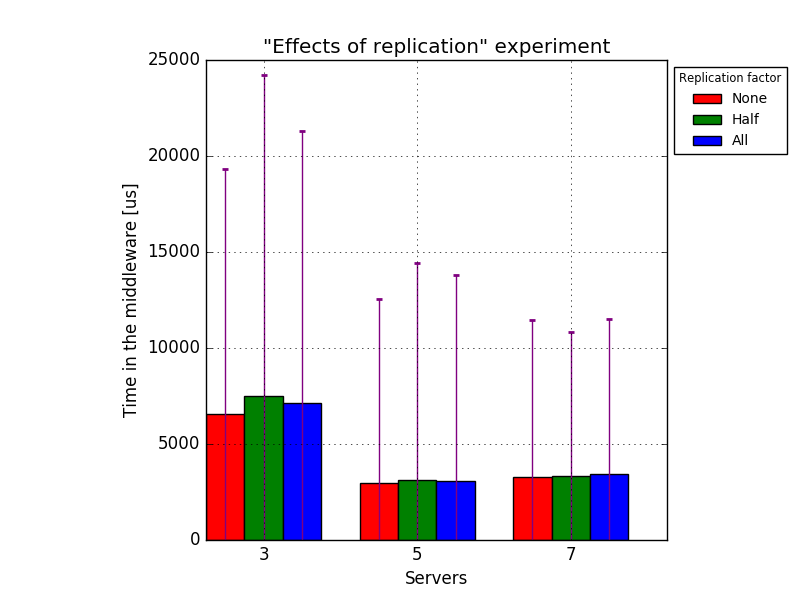
\includegraphics[width=\linewidth]{plots/replication-get-queue}
	\caption{Time in the queue}
\end{subfigure}%
\begin{subfigure}{.5\textwidth}
	\centering
	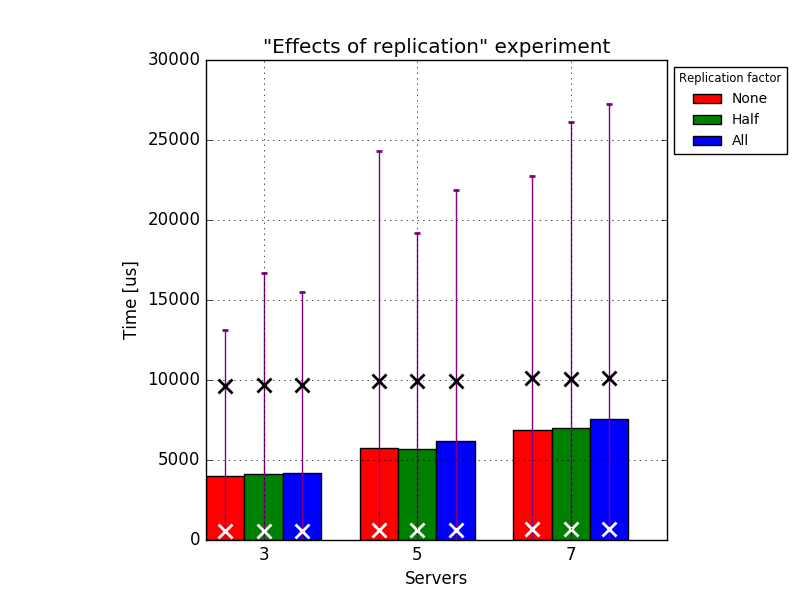
\includegraphics[width=\linewidth]{plots/replication-get-servers}
	\caption{Time in the servers}
\end{subfigure}
\caption{Breakdown of time spent in the middleware for get requests}
\label{fig:replication-get-breakdown}
\end{figure}


\subsection{Set requests}
\begin{figure}
\centering
	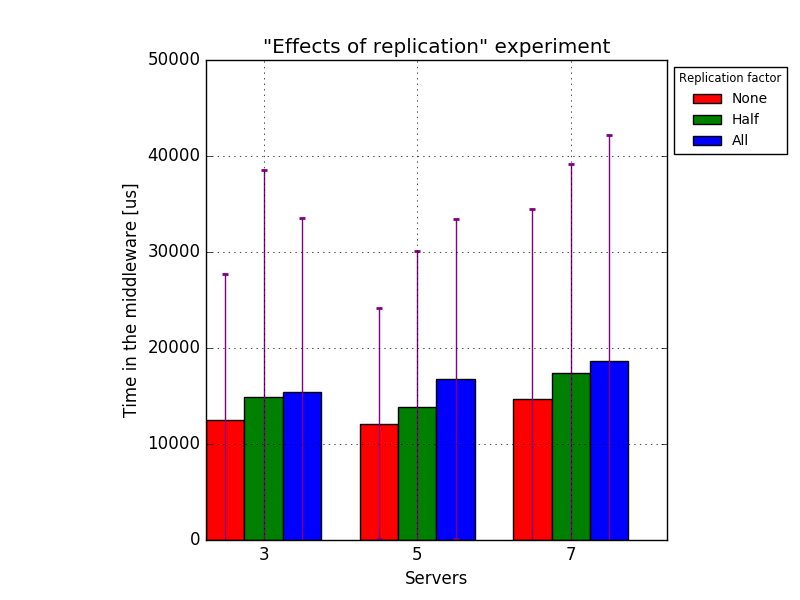
\includegraphics[width=0.7\linewidth]{plots/replication-set}

\caption{Total time spent in the middleware for set requests}
\label{fig:replication-set}
\end{figure}

\begin{figure}
\centering
\begin{subfigure}{.5\textwidth}
	\centering
	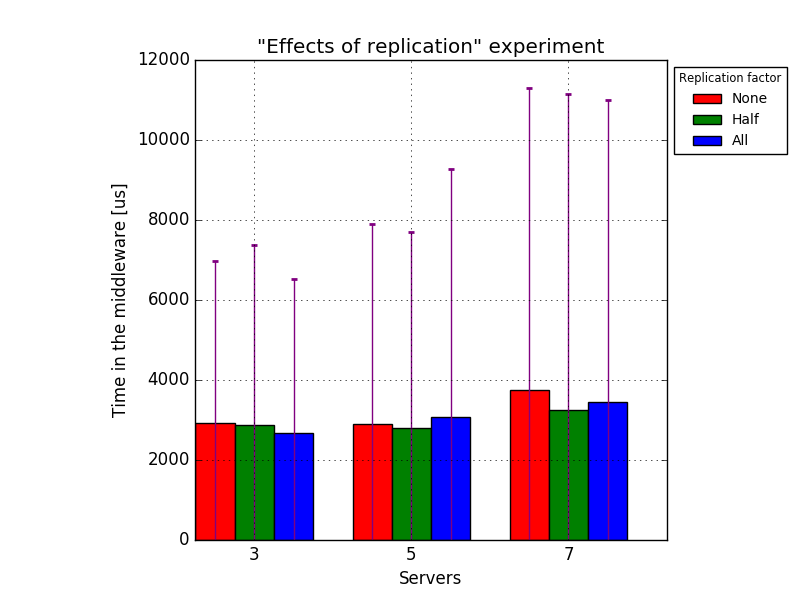
\includegraphics[width=\linewidth]{plots/replication-set-queue}
	\caption{Time in the queue}
\end{subfigure}%
\begin{subfigure}{.5\textwidth}
	\centering
	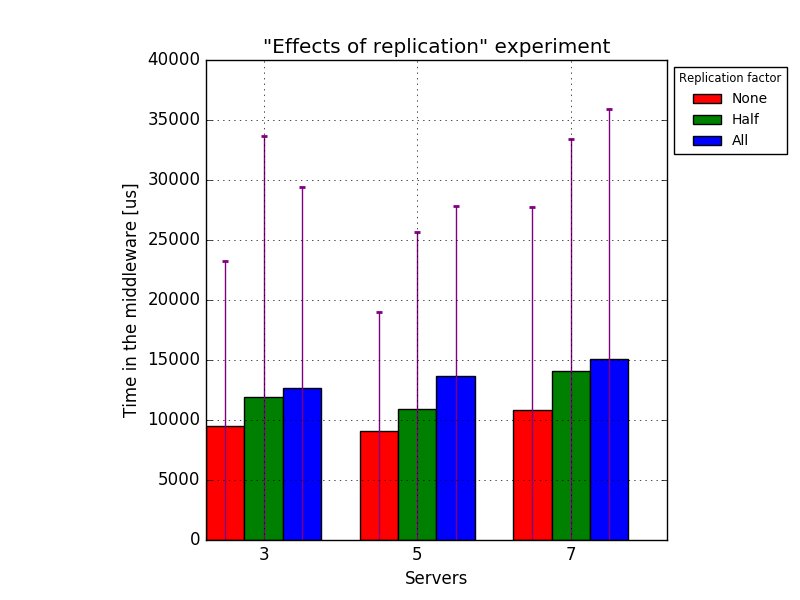
\includegraphics[width=\linewidth]{plots/replication-set-servers}
	\caption{Time in the servers}
\end{subfigure}
\caption{Breakdown of time spent in the middleware for set requests}
\label{fig:replication-set-breakdown}
\end{figure}

\subsection{Get vs set requests}

\subsection{Scalability of the system}

\pagebreak

\section{Effect of Writes}

In this section, you should study the changes in throughput and response time of your system as the percentage of write operations increases. Use a combination of 3 to 7 servers and vary the number of writes between 1\% and 10\% (e.g. 1\%, 5\% and 10\%). The experiments need to be carried out for the replication factors R=1 and R=all.  

For what number of servers do you see the biggest impact (relative to base case) on performance? Investigate the main reason for the reduced performance and provide a detailed explanation of the behavior of the system. Provide the graphs and tables necessary to support your claims.

 
\end{document}